% Prof. Dr. Ausberto S. Castro Vera
% UENF - CCT - LCMAT - Curso de Ci\^{e}ncia da Computa\c{c}\~{a}o
% Campos, RJ,  2021
% Disciplina: Paradigmas de Linguagens de Programa\c{c}\~{a}o
% Aluno: Alysson de Jesus Alcantara



\chapter{ Introdu\c{c}\~{a}o}

\begin{quote}
"As pessoas ainda são loucas pelo Python mesmo depois de vinte e cinco anos,
o que é difícil de acreditar"
—Michael Palin
\end{quote}

Concebido originalmente no final dos anos 80, por por Guido van Rossum no Centrum Wiskunde \& Informatica (CWI) na Holanda, veio como sucessor da linguagem ABC, a implementação se deu inicio em dezembro de 1989. Python foi lançado como sendo uma linguagem de propósito geral de alto nível, multiparadigma, suportando paradigmas orientados a objetos, imperativos, funcionais e procedurais, com uma tipagem dinâmica e de fácil leitura, característica por exigir poucas linhas se comparado a outras linguagens, por conta disso Python é tido como uma das linguagens mais populares da atualidade, considerado a terceira linguagem "mais amada" de acordo com uma pesquisa conduzida pelo site do \href{https://stackoverflow.com/}{Stack Overflow} em 2018 e está entre as 5 linguagens mais populares, de acordo com uma pesquisa conduzida pela RedMonk 

O nome Python teve a sua origem no grupo humorístico britânico Monty Python,[8] criador do programa Monty Python's Flying Circus, embora muitas pessoas façam associação com o réptil do mesmo nome (em português, píton ou pitão).

\begin{quote}
  Em fevereiro de 1991, Van Rossum publicou o código (rotulado como versão 0.9.0) no grupo de discussão da alt.sources. Nessa versão já estavam presentes classes com herança, tratamento de exceções, funções e os tipos de dado nativos \textcolor{purple}{list}, \textcolor{purple}{dict}, \textcolor{purple}{str}, e assim por diante. Também estava presente nessa versão um sistema de módulos emprestado do Modula-3. O modelo de exceções também lembrava muito o do Modula-3, com a adição da opção \textcolor{purple}{else clause}.
  Em 1994 foi formado o principal fórum de discussão do Python, comp.lang.python, um marco para o crescimento da base de usuários da linguagem. \cite{Int01}
\end{quote}

    \newpage
    \section{Aspectos hist\'{o}ricos da linguagem Python}
        
        Python chegou a versão 1.0 em janeiro de 1994. As principais novas funcionalidades incluídas nesta versão foram as ferramentas de programação funcional lambda, map, filtere reduce. Van Rossum afirmou que "Python adquiriu lambda, reduz (), filtro () e mapa (), cortesia de um hacker Lisp que os perdeu e enviou patches de trabalho ". \cite{Int02}
        A última versão lançada enquanto Van Rossum estava no CWI foi o Python 1.2. Em 1995, Van Rossum continuou seu trabalho em Python na Corporation for National Research Initiatives (CNRI) em Reston , Virgínia , de onde lançou várias versões. Abaixo pode-se ver a evolução das logos do Python
        
    \begin{figure}[H]
    \begin{center}
        \caption{Primeira logo da linguagem Python (1990s–2006)} \label{ling1}
        
\includegraphics[width=12cm]{Pictures/primeira-logo-python.png} \\
        {\tiny \sf Fonte: \href{https://commons.wikimedia.org/wiki/File:Python_logo_1990s.svg}{domínio público} }
    \end{center}
   \end{figure}
   

   \begin{figure}[H]
    \begin{center}
        \caption{Logo atual da linguagem python (2006 - atual)} \label{ling1}
        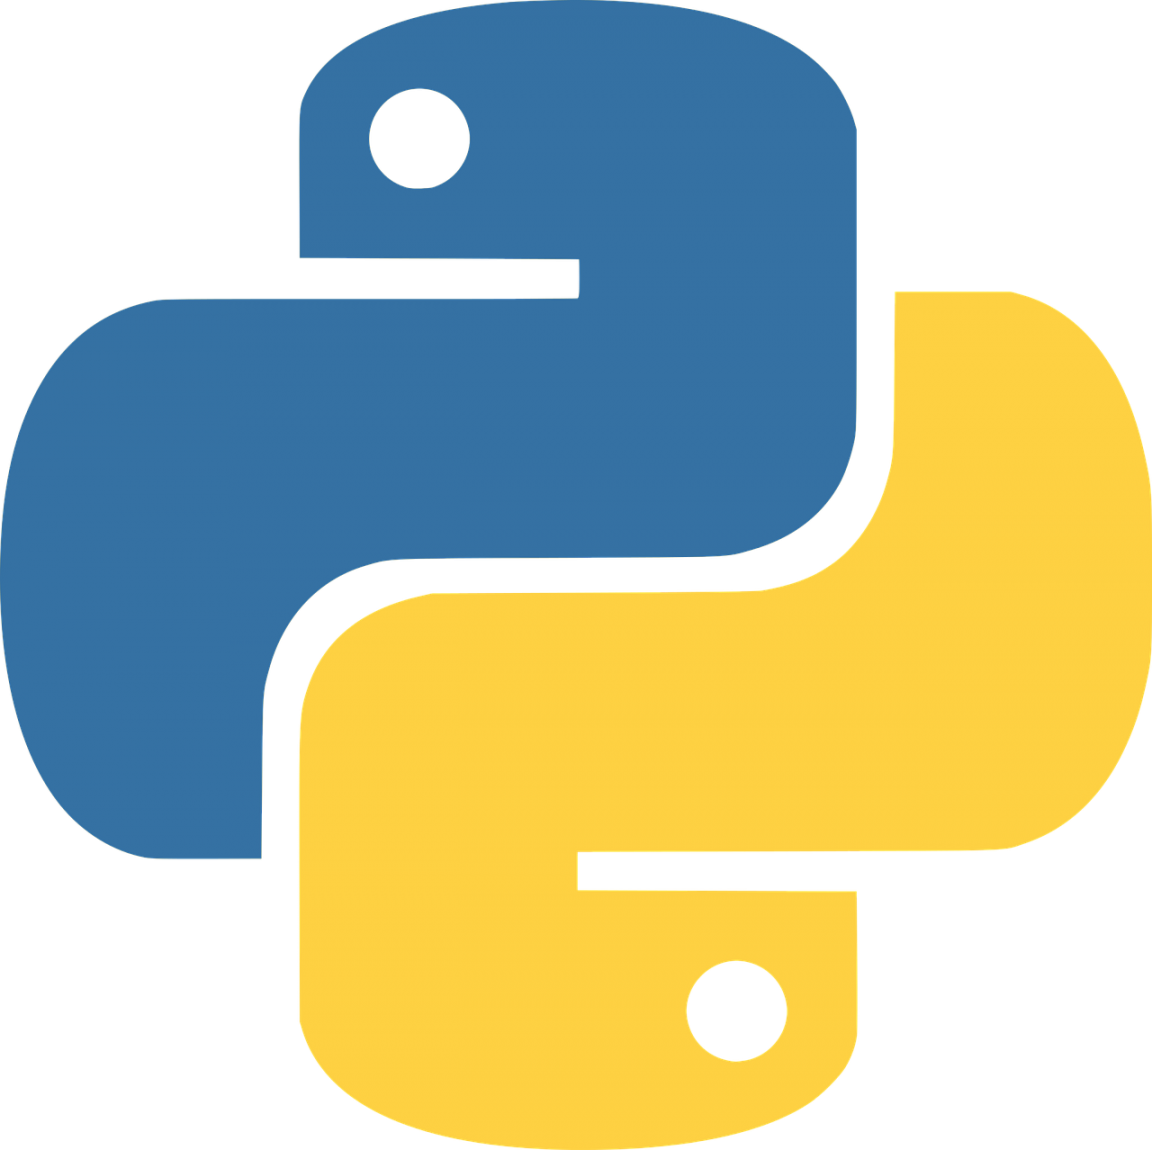
\includegraphics[width=5cm]{python-logo.png} \\
        {\tiny \sf Fonte: \href{https://www.python.org/community/logos/}{community logo python} }
    \end{center}
   \end{figure}
    
   \newpage
   \section{\'{A}reas de Aplica\c{c}\~{a}o da Linguagem}
   
   Por ter uma sintaxe simples e ser baseado em c, Python é uma linguagem que pode ser facilmente escalável e usada em diversas áreas diferentes.
   
   Python pode servir como uma linguagem de script para aplicativos da web, por exemplo, via \textcolor{purple}{mod\_wsgi} para o servidor da web \textcolor{purple}{Apache} Com a Web Server \textcolor{purple}{Gateway Interface}, uma API padrão evoluiu para facilitar essas aplicações. Frameworks da Web como \textcolor{purple}{Django}, \textcolor{purple}{Pylons}, \textcolor{purple}{Pyramid}, \textcolor{purple}{TurboGears}, \textcolor{purple}{web2py}, \textcolor{purple}{Tornado}, \textcolor{purple}{Flask}, \textcolor{purple}{Bottle} e \textcolor{purple}{Zope} apoiam os desenvolvedores no design e manutenção de aplicações complexas. \textcolor{purple}{Pyjs} e \textcolor{purple}{IronPythonpode} ser usado para desenvolver o lado do cliente de aplicativos baseados em \textcolor{purple}{Ajax}. \textcolor{purple}{SQLAlchemy} pode ser usado como um mapeador de dados para um banco de dados relacional. \textcolor{purple}{Twisted}  é um framework para programar comunicações entre computadores e é usado (por exemplo) pelo \textcolor{purple}{Dropbox} \cite{Int03}


        \subsection{ Big Data}
        Python, possui bibliotecas voltada diretamente Big Data, como a Scikit-learn, que oferece funcionalidades para o pré-processamento, a classificação e a clusterização dos dados, a seleção de modelos e a aplicação de algoritmos de regressão.
        Das várias bibliotecas que o python possui para realizar cálculo de Big Data podemos citar a \textcolor{purple}{Imbalanced-learn}, \textcolor{purple}{Jupyter}, \textcolor{purple}{Pandas} e \textcolor{purple}{Scikit-learn}. No artigo de Ivan Eduardo o mesmo realiza uma série de aplicações de Big Data utilizando cada uma das bibliotecas \cite{Int04}
        
        \subsection{ Orienta\c{c}\~{a}o a objetos}
        \cite{Int05} A programação orientada a objetos ( OOP ) é um paradigma de programação baseado no conceito de " objetos ", que podem conter dados e código: dados na forma de campos (geralmente conhecidos como atributos ou propriedades ), e código, na forma de procedimentos (freqüentemente conhecido como métodos ).
        
        Em Python, todo valor é na verdade um objeto. Seja uma tartaruga, uma lista, ou mesmo um inteiro, todos são objetos. Programas manipulam esses objetos realizando computações diretamente com eles ou chamando os seus métodos (ou seja, pedindo que esses objetos executem seus métodos). Para ser mais específico, nós dizemos que um objeto possui um estado e uma coleção de métodos que ele pode executar. O estado de um objeto representa as coisas que o objeto sabe sobre si mesmo. Por exemplo, como vimos com os objetos tartaruga, cada tartaruga possui um estado que representa a sua posição, sua cor, sua direção, etc. Cada tartaruga também tem a capacidade de se mover para a frente, para trás, ou virar para a direita ou esquerda. Cada tartaruga é diferente pois, embora sejam todas tartarugas, cada uma tem um estado diferente (como posições diferentes, ou orientações, etc).
        
        Sabendo como eles funcionam podemos ver um exemplo prático na linguagem python criando um objeto ponto que possui o eixo x e o eixo y
        
    \begin{figure}[H]
    \begin{center}
        \caption{Código de OOP em python, criando um ponto com dois eixos} \label{ling1}
        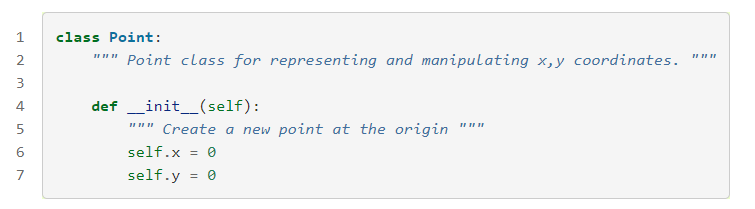
\includegraphics[width=12cm]{Pictures/poo-python.png} \\
        {\tiny \sf Fonte: Autor }
    \end{center}
   \end{figure}
        
        \newpage
        \subsection{ Data Science }
        
        \cite{Int06} Pode-se dizer que um cientista de dados, são para propósitos práticos, estatísticos que entendem sobre ciência da computação, alguns são mais estatísticos e outros são mais engenheiros de software, mas ambos os perfis são cientistas de dados.
        A Ciência de dados serve para extrai todos os dados que estão bagunçados dentro da sociedade, e transforma-los em conhecimento, que servem como guia para melhorar nossa sociedade.
        
        No exemplo abaixo é criado um histograma para agrupar dados unificados em agrupamentos (buckets) discretos e contar quantos pontos vão para cada um, no exemplo esses dados podem representar varias situações como a media diária em minutos que cada usuário passa no seu site.

\subsection*{Trecho de código em python para definir o histograma}
\begin{lstlisting}

def bucketize(point, bucket_size):
"""reduza o ponto para o próximo""" 
"""múltiplo mais baixo de bucket_size"""
return 
    bucket_size * math.floor(point / bucket_size)

def make_histogram(points, bucket_size):
"""agrupa os pontos e conta quantos em cada bucket"""
return 
    Counter(bucketize(point, bucket_size) for point in points)

def plot_histogram(points, bucket_size, title=""):
    histogram = make_histogram(points, bucket_size)
    plt.bar
     (histogram.keys(), histogram.values(), width=bucket_size)
    plt.title(title)
    plt.show()

\end{lstlisting}

\newpage
\subsection*{Agora consideramos os seguintes conjuntos de dados}
\begin{lstlisting}

random.seed(0)
# uniforme entre –100 e 100

uniform = [200 * random.random() - 100 for _ in range(10000)]
# distribuição normal com média 0, desvio padrão 57

normal = [57 * inverse_normal_cdf(random.random())
for _ in range(10000)]

\end{lstlisting}

        Ambos possuem médias próximas a 0 e desvios padrões próximos a 58. No entanto, possuem distribuições bem diferentes. A Figura 10-1 mostra a distribuição de uniform:
        
\begin{lstlisting}
plot_histogram(uniform, 10, "Histograma de Uniform")
\end{lstlisting}
        
        Já o trecho abaixo mostra a distribuição normal
        
\begin{lstlisting}
plot_histogram(normal, 10, "Histograma Normal")
\end{lstlisting}

        Nesse exemplo as duas possuem valores \textcolor{purple}{max} e \textcolor{purple}{min} que podem ser vistos no gráfico abaixo: 
        
    \begin{figure}[H]
    \begin{center}
        \caption{Histograma uniforme} \label{ling1}
        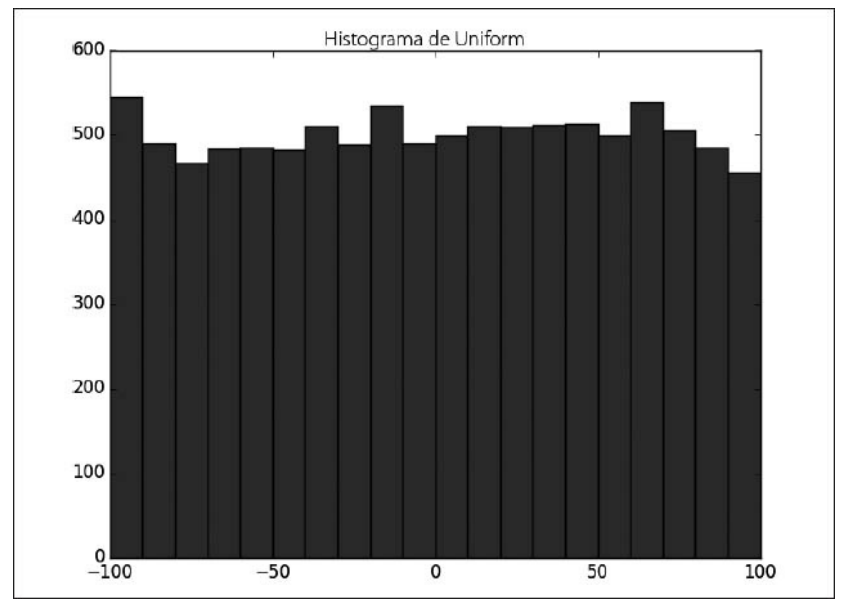
\includegraphics[width=12cm]{Pictures/histograma-grafico.png} \\
        {\tiny \sf Fonte: Livro - Data Science do zero: Primeiras regras com o Python}
    \end{center}
   \end{figure}